	\documentclass[10pt,oneside]{CBFT_book}
	
	% Algunos paquetes
	
	\usepackage{amssymb}
	\usepackage{amsmath}
	\usepackage{graphicx}
	\usepackage{libertine}
	\usepackage{lipsum}
	\usepackage[numbers]{natbib}
	\setcitestyle{square}


	\usepackage{polyglossia}
	\setdefaultlanguage{spanish}

	\usepackage{CBFT.estilo} % Cargo la hoja de estilo
	

	% Tipografías
	% \setromanfont[Mapping=tex-text]{Linux Libertine O}
	% \setsansfont[Mapping=tex-text]{DejaVu Sans}
	% \setmonofont[Mapping=tex-text]{DejaVu Sans Mono}

	%===================================================================
	%	DOCUMENTO PROPIAMENTE DICHO
	%===================================================================

% \title{CBFT Mecánica clásica}
% \author{Mecánica lagrangiana}
% \date{\today}

\begin{document}
% \maketitle
% \tableofcontents
\chapter{Mecánica lagrangiana}

% =================================================================================================
\section{Principio de los trabajos virtuales}
% =================================================================================================
Las ecuaciones de Newton para un sistema de $N$ partículas,
\notamargen{Esto es sumamente sketchi, debemos leer la carpeta de la cursada y luego la
teoría.}
\[
	m_i \vb{a}_i = \vb{F}_i^a + \vb{F}_i^v
\]
dan cuenta de que sobre cada partícula actúan, en principio, fuerzas externas aplicadas $ \vb{F}_i^a $
y fuerzas de vínculo $ \vb{F}_i^v $. Expresando la aceleración en función de la derivada temporal del momento  
$ \dot{\vb{p}}_i = m_i \vb{a}_i$ resulta 
\[
	\dot{\vb{p}}_i - \vb{F}_i^a - \vb{F}_i^v = 0,
\]
y entonces, multiplicando cada término por un desplazamiento virtual $ \delta\vb{x}_i $ se tiene
\[
	\sum_i^N \left( \dot{\vb{p}}_i - \vb{F}_i^a - \vb{F}_i^v \right) \cdot \delta\vb{x}_i  = 0.
\]

\notamargen{Explicar qué es este principio y qué es un desplazamiento virtual.}
Si hacemos estos desplazamientos son {\it compatibles} con los vínculos nos quedamos con
\be
	\sum_i^N \left( \dot{\vb{p}}_i - \vb{F}_i^a \right) \cdot \delta\vb{x}_i = 0,
% 	- \sum_i^N  \vb{F}_i^v  \cdot \delta\vb{x}_i  = 0
	\label{principio_virtual_work}
\ee
puesto que las fuerzas de vínculo son siempre perpendiculares a los desplazamientos virtuales, es decir 
\[
	\vb{F}_i^v \perp \delta\vb{x}_i.
\]

La expresión \eqref{principio_virtual_work} es el llamado {\it Principio de los Trabajos Virtuales},
y dada la independencia admitida en los desplazamientos virtuales $ \delta \vb{x}_i $, se sigue que 
\[
	\dot{\vb{p}}_i - \vb{F}_i^a = 0 \quad \forall i
\]

\begin{notas}{Relación vínculos y desplazamientos:}
El hecho de que la fuerza de vínculo sea perpendicular a los desplazamientos puede
verse a partir de que la ecuación de vínculo en un sistema toma la forma
\notamargen{¿Y esta magia? Hay que aclarar realmente que sea así como se dice que es.}
\[
	f(\vb{r}_i) - K = 0 
\]
luego, derivando implícitamante cada ecuación y sumando (si se nos permite un pequeño
abuso de notación)
\[
	\sum_i^N \dpar{f}{\vb{r}_i} d\vb{r}_i = 0 
\]
pero esto no es otra cosa que
\[
	\nabla f \cdot \vb{\delta r} = 0
\]
donde debemos entender al gradiente y al vector $\vb{\delta r}$ como $N$ dimensionales.
\end{notas}

% =================================================================================================
\section{Construcción del lagrangiano}
% =================================================================================================

Consideremos un sistema de $N$ partículas, $k$ ecuaciones de vínculo y por ende $3N - k$ grados de libertad
(estamos en 3 dimensiones).

Tenemos $N$ relaciones
\[
	\vb{r}_i = \vb{r}_i(q_1,q_2,...,q_{3N-k},t)
\]
entonces una variación serán
\[
	\delta \vb{r}_i =  \sum_{j=1}^{3N-k} \left( \dpar{\vb{r}_i}{q_j} \right) \delta q_j + 
	\dpar{\vb{r}_i}{t}\delta t
\]
donde el último $\delta t$ es nulo por ser un desplazamiento virtual de manera que
\[
	\delta \vb{r}_i =  \sum_{j=1}^{3N-k} \left( \dpar{\vb{r}_i}{q_j} \right) \delta q_j.
\]

Por otro lado
\[
	\sum_i^N \dot{\vb{P}}_i \cdot \delta \vb{r}_i - \sum_i^N  \vb{F}_i^a \cdot \delta \vb{r}_i = 0
\]
y se puede reescribir el primer término como
\[
	\dot{\vb{P}}_i \cdot \delta \vb{r}_i = m_i \dtot{\vb{v}_i}{t}\sum_{j=1}^{3N-k} 
	\left( \dpar{\vb{r}_i}{q_j} \right) \delta q_j
\]
resultando
\[
	\sum_i^N m_i \dtot{\vb{v}_i}{t} \cdot \sum_{j=1}^{3N-k} \left( \dpar{\vb{r}_i}{q_j} \right)
	\delta q_j - \sum_i^N  \vb{F}_i^a \cdot \delta \vb{r}_i = 0
\]

La idea ahora es reescribir todo en términos más convenientes, para que aparezca un término multiplicado
a una variación arbitraria. De esta manera quedará una sumatoria de un sumando multiplicado por una
variación igualada a cero. No cabe otra posibilidad que el sumando sea nulo para cada índice de la suma.
\notamargen{Escrito muy mal este texto. La idea es clara, no obstante: hay que purificarla}

Consideremos la derivada total de 
\[
	\frac{d}{dt}\left( m_i\vb{v}_i\dpar{\vb{r}_i}{q_j} \right) =
	m_i \dtot{\vb{v}_i}{t}\dpar{\vb{r}_i}{q_j} + m_i \vb{v}_i \frac{d}{dt}\left(\dpar{\vb{r}_i}{q_j}\right).
\]
Pero la diferencial del vector $\vb{r}_i$ es (notemos que no es una variación)
\[
	d\vb{r}_i = \sum_{j=1}^{3N-k} \left( \dpar{\vb{r}_i}{q_j} \right) dq_j + \dpar{\vb{r}_i}{t} dt
\]
y entonces
\[
	\dot{\vb{r}}_i = \vb{v}_i = \sum_{j=1}^{3N-k} \left( \dpar{\vb{r}_i}{q_j} \right)
	\dot{q}_j + \dpar{\vb{r}_i}{t}.
\]
La derivada de la velocidad de la partícula $i$-ésima respecto a la coordenada $l$-ésima es
\[
	\dpar{\vb{v}_i}{\dot{q}_l} = \dpar{\vb{r}_i}{q_l} =
	\frac{\partial \vb{r}_i/\partial t}{\partial q_l/\partial t}.
\]
Si derivamos nuevamente
\[
	\frac{\partial}{\partial q_l} \left( \dtot{\vb{r}_i}{t} \right) =
	\dpar{\vb{v}_i}{q_l} = \sum_{j=1}^{3N-k} \dparcru{\vb{r}_i}{q_j}{q_l} \dot{q}_j + 
	\dparcru{\vb{r}_i}{t}{q_l}.
\]
\[
	\frac{d}{dt} \left( \dpar{\vb{r}_i}{q_l} \right) = 
	\frac{d}{dt} \left( \sum_{j=1}^{3N-k} \dparcru{\vb{r}_i}{q_j}{q_l} dq_j +
	\dparcru{\vb{r}_i}{t}{q_l} dt \right) 
\]
de tal manera que 
\[
	\frac{d}{dt} \left( \dpar{\vb{r}_i}{q_l} \right) = \dpar{\vb{v}_i}{q_l}
\]

Volvemos ahora a la eq III y 
\[
	\sum_i^N \sum_{j=1}^{3N-k} \left[ 
	\frac{d}{dt} \left( m_i \vb{v}_i \dpar{\vb{r}_i}{q_j} \right) - 
	m_i \vb{v}_i \frac{d}{dt}\left( \dpar{\vb{v}_i}{q_j} \right) \right] \delta q_j
\]
y este corchete lo reescribimos como 
\[
	\sum_i^N \sum_{j=1}^{3N-k} \left[ 
	\frac{d}{dt} \left( m_i \vb{v}_i \dpar{\vb{v}_i}{\dot{q}_j} \right) -
	m_i \vb{v}_i \dpar{\vb{v}_i}{q_j} \right] \delta q_j
\]

\[
	\sum_i^N \sum_{j=1}^{3N-k} \left\{ 
	\frac{d}{dt} \left[ \frac{\partial}{\partial \dot{q}_j} \left( \frac{m_i}{2} \vb{v}_i^2 \right) \right] - 
	\frac{\partial}{\partial q_j} \left( \frac{m_i}{2} \vb{v}_i^2 \right) \right\} \delta q_j
\]

Ahora introducimos la sumatoria en $i$ hacia adentro de ambos términos,
\[
	\sum_{j=1}^{3N-k} \left\{ 
	\frac{d}{dt} \left[ \frac{\partial}{\partial \dot{q}_j}
	\left( \sum_i^N \frac{m_i}{2} \vb{v}_i^2 \right) \right] 
	-  \frac{\partial}{\partial q_j} \left( \sum_i^N \frac{m_i}{2} \vb{v}_i^2 \right) \right\} \delta q_j
\]
de modo que dentro de los paréntesis resulta $T$, luego 
\[
	\sum_i^N \dot{\vb{P}}_i \cdot \delta \vb{r}_i = 
	\sum_{j=1}^{3N-k} \left\{ \frac{d}{dt} \left[ \frac{\partial}{\partial \dot{q}_j} \left( T \right) \right] - 
	\frac{\partial}{\partial q_j} \left( T \right) \right\} \delta q_j
\]
\[
	\sum_i^N \dot{\vb{P}}_i \cdot \delta \vb{r}_i = 
	\sum_{j=1}^{3N-k} \sum_i^N \vb{F}_i^a \cdot \dpar{\vb{r}_i}{q_j} \delta q_j =  
	\sum_{j=1}^{3N-k} \sum_i^N Q_j \delta q_j
\]
siendo $Q_j$ la fuerza generalizada. Entonces
\[
	\sum_{j=1}^{3N-k} \left\{ \frac{d}{dt}
	\left[ \frac{\partial}{\partial \dot{q}_j} \left( T \right) \right] - \frac{\partial}{\partial q_j}
	\left( T \right) - Q_j \right\} \delta q_j =  0.
\]

Si suponemos que las fuerzas son conservativas entonces 
\[
	Q_j \delta q_j = -\dpar{V}{q_j}\delta q_j
\]
y como $V=V(\vb{r}_1,...,\vb{r}_n)$ se tiene 
\[
	V = \sum_i^N  \dpar{V}{r_i} \delta \vb{r}_i = \dpar{V}{\vb{r}_i} \cdot \dpar{\vb{r}_i}{q_j} \delta q_j =
\]
pero 
\[
	Q_j = - \dpar{V}{q_j}
\]
y entonces 
\[
	\sum_{j=1}^{3N-k} \left\{ 
	\frac{d}{dt} \left( \dpar{T}{\dot{q}_j} \right) - \frac{\partial}{\partial q_j}
	\left( T - V \right) \right\} \delta q_j =  0.
\]

Definimos como 
\[
	\Lag \equiv T - V
\]
y entonces podemos escribir
\[
	\sum_{j=1}^{3N-k} \left[
	\frac{d}{dt} \left( \dpar{\Lag}{\dot{q}_j} \right) -  \dpar{\Lag}{q_j} \right] \delta q_j =  0.
\]

Si existieran fuerzas que no provienen de un potencial entonces
\[
	Q_j + Q_j^{NC} = -\dpar{V}{q_j} + Q_j^{NC}
\]
y finalmente 
\[
	\sum_{j=1}^{3N-k} \left[
	\frac{d}{dt} \left( \dpar{\Lag}{\dot{q}_j} \right) -  \dpar{\Lag}{q_j} \right] \delta q_j = 
	\sum_{j=1}^{3N-k} Q_j^{NC} \delta q_j
\]

Como esto vale para todo grado de libertad $l$ llegamos a
\[
	\frac{d}{dt} \left( \dpar{\Lag}{\dot{q}_j} \right) -  \dpar{\Lag}{q_j} = Q_j^{NC}
\]
que son las ecuaciones de Euler-Lagrange. Este es el resultado más importante del capítulo.

% =================================================================================================
\section{Invariancia del lagrangiano ante adición de una derivada total}
% =================================================================================================

Sea una función de las coordenadas y del tiempo $F=F(q_i,t)$ que sumamos al lagrangiano $\Lag$, de modo que
\[
	\Lag'=\Lag + \dtot{F}{t} 
\]
y las ecuaciones de Euler-Lagrange para este nuevo lagrangiano son
\[
	\frac{d}{dt}\left(\dpar{\Lag'}{\dot{q}_j}\right) - \dpar{\Lag'}{q_j} = 0
\]
\[
	\dtot{}{t}\left(\dpar{\Lag}{\dot{q}_j} + \dpar{}{\dot{q}_j}\left(\dtot{F}{t}\right)\right) -
	\dpar{\Lag}{q_j} - \dpar{}{q_j}\left( \dtot{F}{t}\right) = 0 
\]
\[
	\dtot{}{t}\left(\dpar{\Lag}{\dot{q}_j}\right) - \dpar{\Lag}{q_j} + 
	\dtot{}{t}\left(\dpar{}{\dot{q}_j}\left(\dtot{F}{t}\right)\right) 
	- \dpar{}{q_j}\left( \dtot{F}{t}\right) = 0 
\]

Ahora es necesario escribir la derivada total de $F$,
\[
	\dtot{F}{t} = \sum_j^{3N-k} \dpar{F}{q_j}\dtot{q_j}{t} + \dpar{F}{t} =
			\sum_j^{3N-k} \dpar{F}{q_j}\dot{q}_j + \dpar{F}{t}
\]
y ver que
\[
	\dpar{}{\dot{q}_j}\left(\dtot{F}{t}\right) = \dpar{F}{q_j} \qquad\qquad
	\dpar{}{q_j}\left(\dtot{F}{t}\right) = \dpar[2]{F}{q_j} \dot{q}_j + \dparcru{F}{t}{q_j} 
\]

Luego, usando esta información, resulta que los términos que surgen de la adición de la derivada total de $F$ resultan 
ser
\[
	\dtot{}{t}\left( \dpar{}{\dot{q}_j}\left(\dtot{F}{t}\right)\right) - 
	\dpar{}{q_j}\left( \dtot{F}{t}\right) = \dtot{}{t}\left( \dpar{F}{q_j} \right) - 
	\dpar{}{q_j}\left( \dtot{F}{t}\right)
\]
\[
	\dtot{}{t}\left( \dpar{F}{q_j} \right) - \dpar{}{q_j}\left( \dtot{F}{t}\right) =
	\dpar[2]{F}{q_j} \dot{q}_j + \dparcru{F}{q_j}{t} - \dpar{}{q_j}\left( \dtot{F}{t}\right)
\]
y si aceptamos que $F$ es de clase C$^2$ se tiene
\[
	\dpar[2]{F}{q_j} \dot{q}_j + \dparcru{F}{q_j}{t} - \dpar{}{q_j}\left( \dtot{F}{t}\right)=0
\]
de modo que las ecuaciones de Euler Lagrange no se modifican si añadimos una derivada total respecto del tiempo de una 
función de $q_j,t$.

% =================================================================================================
\section{Momentos conjugados y coordenadas cíclicas}
% =================================================================================================

Dado un lagrangiano $\Lag = \Lag( q_i,\dot{q}_i, t )$ se define el momento canónicamente conjugado a $q_j$
como 
\be
	p_j \equiv \dpar{\Lag}{\dot{q}_j},
	\label{mom_canon_conj}
\ee
y entonces 
\[
	\dot{p}_j = \frac{d}{dt}\left( \dpar{\Lag}{\dot{q}_j} \right) \equiv Q_j,
\]
que es la fuerza generalizada en el grado de libertad $j$.

Sea ahora un lagrangiano que no depende explícitamente de la coordenada $k$, es decir 
\[
	\Lag = \Lag( q_1,...,q_{k-1},q_{k+1},...,q_n,\dot{q}_1,...\dot{q}_n, t ),
\]
entonces será
\[
	\dpar{\Lag}{q_k}= 0 
\]
y como consecuencia las ecuaciones de Euler-Lagrange en la coordenada $k$-ésima resultan 
\[
	\dtot{}{t}\left( \dpar{\Lag}{\dot{q}_k} \right) = \dot{ p }_k = Q_k = 0 
% 	\quad \rightarrow \;\dot{p}_k = 0 \quad \rightarrow \; p_k = cte.
\]
de manera que no existe fuerza generalizada en el grado de libertad $k$ y como es $\dot{p}_k = 0$, se conserva 
el momento $p_k$ canónicamente conjugado a $q_k$.
En estos casos se dice que la coordenada $q_k$ que no aparece en el lagrangiano, es una coordenada
cíclica.

\begin{ejemplo}{\bf Potencial central en un plano}

Sea un potencial central $ V(r) $ en el plano. El lagrangiano de una partícula de masa $m$ sometida al mismo,
y en las convenientes coordenadas polares $(r,\vp)$ es
\[
	\Lag = \frac{1}{2} m ( \:\dot{r}^2 + r^2 \dot{\vp}^2 ) - V(r).
\]
Luego, las ecuaciones de Euler-Lagrange serán, en $r$,
\[
	\dtot{}{t}\left( \dpar{\Lag}{\dot{r}}\right) - \dpar{\Lag}{r} =
	m\ddot{r} - m\dot{\vp}^2r + \dtot{V}{r} = 0
\]
y en $\vp$
\[
	\dtot{}{t}\left( \dpar{\Lag}{\dot{\vp}}\right) = mr^2\ddot{\vp} = 0.
\]
En esta última debemos notar que $\partial \Lag / \partial \vp = 0 $ y esto significa que $\vp$ es cíclica.
Entonces se conserva el momento canónicamente conjugado a $\vp$ puesto que verifica 
\[
	\dot{p}_\vp = mr^2\ddot{\vp} = 0
\]
lo cual lleva a que $ m r^2\dot{\vp} $ es una constante para este sistema. La moraleja es que la existencia de una 
coordenada cíclica permite ahorrarnos una integración.
Esto, por supuesto, para este problema no es otra cosa que la conservación del momento angular [?].

\end{ejemplo}

% =================================================================================================
\section{Momentos canónicamente conjugados y traslaciones rígidas}
% =================================================================================================

Consideremos un sistema de partículas que sufre una traslación rígida infinitesimal.
Esta traslación se lleva a cabo a través de un desplazamiento en la coordenada $ q $ y de magnitud 
$\delta q$ en la dirección dada por el versor $ \hat{n} $.
% Esta coordenada justamente tiene esa propiedad: una variación de ella representa una 
% traslación rígida.
% ESTE COMENTARIO, que estaba en la carpeta, ahora queda un poco desplazado por la sentencia más
% correcta con respecto a la dirección \hat{n}. Supongo que lo importante es la dirección que en
% el caso de cartesianas la da la misma q pero que en el caso de versores que varían su dirección
% curvilíneos, debe especificarse.

En efecto, para el sistema de $ N $ partículas, la traslación rígida implica
\[
	q \longrightarrow q + \delta q \qquad 
	\vb{x}_i \longrightarrow \vb{x}_i + \delta q \; \hat{n}
\]
La Figura \ref{traslacion_rigida} representa la situación.

Luego, suponiendo una energía cinética de tipo $T_2$, el momento canónicamente conjugado $ p $ (en 
la coordenada $q$ --cuyo subíndice omitimos--) es
\notamargen{[¿se sabe esto a esta altura?]}
\[
	p = \dpar{T}{\dot{q}} = \frac{1}{2} \sum_i^N m_i \left( \dpar{\vb{v}_i^2}{\dot{q}}\right) =
	\sum_i^N m_i \vb{v}_i \cdot \dpar{\vb{v}_i}{\dot{q}} 
\]
\notamargen{Hablar de vectores al cuadrado.\\}
\notamargen{\\ Nota de cómo se manipula: uso $dv^2_i = 2 v_i dv_i$ y}

La {\it forma} de la traslación rígida implica que 
\[
	\dpar{\vb{v}_i}{\dot{q}} = \dpar{\vb{x}_i}{q} = 
	\lim_{\delta q \to 0} \frac{\vb{x}_i + \delta q \:\hat{n} -\vb{x}_i}{\delta q} = \hat{n}.
\]
\notamargen{Recodemos que $ \vb{v}_i = \dot{q}_j\dpar{\vb{x}_i}{q_j} - \dpar{\vb{x}_i}{t} $ }
de modo que 
\[
	p = \sum_i^N m_i \vb{v}_i \cdot \hat{n} = \left( \sum_i^N m_i \vb{v}_i \right) \cdot \hat{n} 
	= \vb{P} \cdot \hat{n} = P_{\hat{n}}
\]

\begin{figure}[htb]
	\begin{center}
	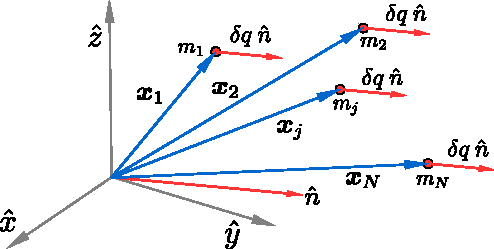
\includegraphics[width=0.6\textwidth]{images/fig_mc_tras_rig.pdf}	 
	\end{center}
	\caption{}
	\label{traslacion_rigida}
\end{figure} 

Hemos arribado al resultado de que el momento canónicamente conjugado correspondiente a la coordenada
generalizada asociada a la traslación rígida es la proyección del momento total en la dirección de ésta.

Para el ejemplo trivial de la partícula libre, $T = 1/2 \; m (\dot{x}^2+ \dot{y}^2+\dot{z}^2)$, se
tiene $ p_x = m v_x $ si la traslación es en la dirección $ \hat{x} $.
\notamargen{Este ejemplo suma algo?}

Para las fuerzas generalizadas, equivalentemente se tiene 
\[
	Q = \sum_i^N \vb{F}^a_i \cdot \dpar{\vb{x}_i}{q} =
	\left( \sum_i^N \vb{F}^a_i \right) \cdot \hat{n} = \vb{F}\cdot \hat{n},
\]
la fuerza generalizada es la proyección de las fuerzas aplicadas en la dirección dada por $ \hat{n} $.

\notamargen{Revisar porque esto no estaba tan claro. Supongo que la idea es ver que aún con presencia
de $T_1$ esto sigue valiendo}
La ecuación para la fuerza generalizada $Q_j$ era
\[
	Q_j = \frac{d}{dt}\left( \dpar{T}{\dot{q}_j} \right) - \dpar{T}{q_j}.
\]
Aún en el caso de que $T$ dependa de $q_j$ la traslación rígida implica que 
$ \partial{T}/\partial{q_j} = 0 $ 
porque es sumar un vector constante a la posición, luego $ d\vb{x}_i/dt = d(\vb{x}_i + \vb{a}) /dt$
para todo \vb{a} constante. Entonces, para la coordenada q asociada a la traslación en $\hat{n}$
se tiene 
% \[
% 	Q_j = \frac{d}{dt}\left( \dpar{T}{\dot{q}_j} \right)
% \]
% y en el caso de la traslación con dirección $\hat{n}$,
\[
	Q = \frac{d}{dt}\left( \dpar{T}{\dot{q}} \right) = \dtot{P_{\hat{n}}}{t},
\]
de tal manera que si en $\hat{n}$ no hay fuerza $Q$ tendremos $ d P_{\hat{n}}/dt = 0 $, es decir 
$ P_{\hat{n}} $ conservado.

\notamargen{Acá la cosa es que la traslación es una cosa que sufre el sistema pero no es dinámica.
Es una construcción nuestra, como un cambio de sistema de referencia.}

% pero el segundo término del lado izquierdo $\partial T/\partial q_j = 0$ puesto que la $T$ no se ve
% afectada por cambiar trasladando rígidamente el sistema.
% \[
% 	\frac{d}{dt}(\vb{p}\cdot \hat{n}) = \vb{F}\cdot \hat{n},
% \]
% y esto significa que el $p_j$ se conserva si no hay fuerza en $\hat{j}$.

% =================================================================================================
\section{Momentos canónicamente conjugados y rotaciones rígidas}
% =================================================================================================

Ahora consideraremos un sistema de partículas que sufre una rotación rígida infinitesimal.
Esta se materializa a través de un desplazamiento angular en la coordenada $ q $ de magnitud $\delta q$.
La dirección y sentido, para cada posición $ \vb{x}_i $ vienen dadas por el producto vectorial 
$ \hat{n} \times \vb{x}_i$.

\notamargen{Esta coordenada $q$ es especial en el sentido en que representa una rotación.}
Para un sistema de $ N $ partículas, la rotación rígida implica
\[
	q \longrightarrow q + \delta q |\vb{x}| \sin \alpha_i \qquad
	\vb{x}_i \longrightarrow \vb{x}_i + \delta q \; \hat{n} \times \vb{x}_i
\]
La Figura \ref{rotacion_rigida} representa la situación, donde por razones de claridad se muestran
solamente dos partículas.

\begin{figure}[htb]
	\begin{center}
	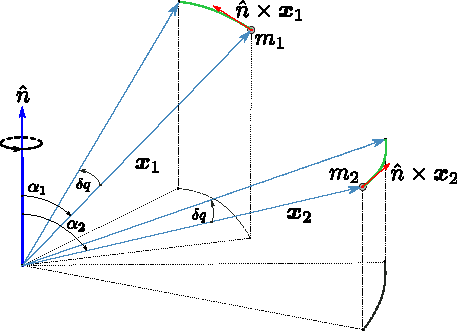
\includegraphics[width=0.6\textwidth]{images/fig_mc_rot_rig.pdf}	 
	\end{center}
	\caption{}
	\label{rotacion_rigida}
\end{figure} 
% Ahora es el turno de la rotación rígida. Sea coordenada que representa rotación rígida,
% \[
% 	\vb{r}_i \longrightarrow \vb{r}_i + \delta q (\hat{n} \times \vb{r}_i)
% \]
El momento canónicamente conjugado en la coordenada angular $q$ será
\[
	p = \dpar{T}{\dot{q}} = 
	\sum_i^N m_i \vb{v}_i \cdot \dpar{\vb{v}_i}{\dot{q}} =
	\sum_i^N m_i \vb{v}_i \cdot \hat{n} \times \vb{x}_i = 
	\sum_i^N m_i \vb{v}_i \cdot ( \hat{n} \times \vb{x}_i )
\]
donde hemos utilizado el hecho de que 
\[
	\dpar{\vb{v}_i}{\dot{q}} = \dpar{\vb{x}_i}{q} = 
	\lim_{\delta q \to 0} \frac{ \vb{x}_i +\delta q (\hat{n} \times \vb{x}_i)- 
	\vb{r}_i}{\delta q} = \hat{n} \times \vb{x}_i. 
\]

El sumando se puede reescribir (usando $\vb{A}\cdot(\vb{B}\times\vb{C}) = 
\vb{B}\cdot(\vb{C}\times\vb{A})$) para que aparezca explícitamente la forma buscada,
\[
	p = \sum_i^N m_i \vb{v}_i \cdot ( \hat{n} \times \vb{x}_i ) =
	\sum_i^N \hat{n} \cdot ( \vb{x}_i \times m_i \vb{v}_i  ) =
	\sum_i^N \hat{n} \cdot \vb{l}_i = \hat{n} \cdot \sum_i^N \vb{l}_i =
	\hat{n} \cdot \vb{L}
\]
que significa
\[
	p = \hat{n} \cdot \vb{L} = L_{\hat{n}},
\]
el momento canónicamente conjugado en la dirección $\hat{n}$ es el momento angular total
del sistema proyectado en esa dirección.
% \[
% 	|\delta q(\hat{n} \times \vb{r}_i)| = \delta q r_i \sin (\alpha)
% \]
% El momento canónicamente conjugado en la dirección $\hat{n}$ es el $\vb{L}$ proyectado en esa dirección.
% \[
% 	\frac{d}{dt}(\hat{n}\cdot\vb{L}) = \hat{n}\cdot\vb{\tau}
% \]
% y el $p_j$ se conserva si no hay torque.
La fuerza generalizada será
\[
	Q = \sum_i^N \vb{F}^a_i \cdot \dpar{\vb{x}_i}{q} = 
	\sum_i^N \vb{F}^a_i \cdot ( \hat{n} \times \vb{x}_i ) = 
	\hat{n} \cdot \left( \sum_i^N \vb{x}_i \times  \vb{F}^a_i \right) = 
	\hat{n} \cdot \sum_i^N \vb{\tau}_i = \hat{n} \cdot \vb{\Tau},
\]
i.e. la componente del torque en la dirección $ \hat{n} $.

Asimismo, si la coordenada implica una rotación rígida entonces $ \partial{T}/\partial{q} = 0 $ 
debido a que la energía cinética $ T $ es un escalar y es por ende invariante ante rotaciones
(un vector rotado cambia su dirección pero no su módulo).
Luego
\[
	Q = \frac{d}{dt}\left( \dpar{T}{\dot{q}} \right) = \dtot{L_{\hat{n}}}{t} = \vb{\Tau}_{\hat{n}}.
\]
% \[
% 	\frac{d}{dt}\left( \hat{n}\cdot \vb{L} \right) = \hat{n}\cdot \vb{\tau}
% \]
\notamargen{Tal vez un ejemplo 2D ayude a aclarar un poco este tema.}

Todo este análisis (traslaciones y rotaciones rígidas) vale si el potencial $V$ no depende de la
velocidad; en caso contrario cambia la forma de los momentos canónicos. En efecto, en este caso
es
\[
	p = \dpar{ \Lag }{\dot{q}} = \dpar{(T-V)}{\dot{q}}
\]
Volviendo al ejemplo de la partícula de masa $m$ y carga $q$ en un campo electromagnético se tendrá
\[
	p = m v_{\hat{n}} + \frac{q}{c} \vb{A}\cdot\hat{n},
\]
es decir que aparece un término extra con el potencial vector respecto del caso en que la partícula
está libre.

% =================================================================================================
\section{Energía cinética de un sistema}
% =================================================================================================

Resulta útil disponer de la energía cinética de un sistema en función de coordenadas generalizadas.
Para un sistema de $N$ partículas, es 
\[
	T = \frac{1}{2} \sum_i^N m_i |\vb{v}_i|^2 
\]
donde las posiciones de cada una de ellas se pueden expresar en términos de $k$ coordenadas generalizadas
\[
	\vb{x}_i = \vb{x}_i(q_1, q_2, ..., q_k, t )
\]
y sus respectivas velocidades serán
\notamargen{La derivada con respecto al tiempo de la posición es la $ d/dt $ no la parcial.}
\[
	\vb{v}_i = \sum_j^{k}  \dpar{\vb{x}_i}{q_j} \: \dot{q}_j + \dpar{\vb{x}_i}{t}.
\]
\notamargen{Este chapter es básicamente un desarrollo formal, habría que bajar con alguna aplicación práctica.}
Luego, utilizando el hecho de que $ |\vb{v}_i|^2 = \vb{v}_i \cdot \vb{v}_i $, se tiene 
\be
	T = \frac{1}{2} \sum_i^N m_i \left( \sum_{j=1}^{k}  \dpar{\vb{x}_i}{q_j}\dot{q}_j + \dpar{\vb{x}_i}{t} \right)
	\cdot \left( \sum_{s=1}^{k} \dpar{\vb{x}_i}{q_s}\dot{q}_s + \dpar{\vb{x}_i}{t} \right) 
\label{mc_T}
\ee
y expandiendo el producto resulta
\[
	T = \frac{1}{2} \sum_i^N m_i \left[ \sum_j^{k}\sum_s^{k} \dpar{\vb{x}_i}{q_j} \cdot \dpar{\vb{x}_i}{q_s}\dot{q}_s\dot{q}_j + 
	2 \dpar{\vb{x}_i}{t} \cdot \sum_j^{k} \dpar{\vb{x}_i}{q_j}\dot{q}_j + \left| \dpar{\vb{x}_i}{t} \right|^2 \right],
\]
la cual se puede separar en tres contribuciones
\[
	T = T_2 + T_1 + T_0
\]
\notamargen{Sacarle espacio al \texttt{cdot}}
con las siguientes formas:
\[
	T_2 = \frac{1}{2} \sum_j^{k} \sum_s^{k} \left( \sum_i^N m_i \dpar{\vb{x}_i}{q_j} \cdot \dpar{\vb{x}_i}{q_s} \right) \dot{q}_j\dot{q}_s
\]
\[
	T_1 =  \sum_j^{k} \left( \sum_i^N m_i \dpar{\vb{x}_i}{t} \cdot \dpar{\vb{x}_i}{q_j} \right) \dot{q}_j
\]
\[
	T_0 = \frac{1}{2} \sum_i^N m_i \left| \dpar{\vb{x}_i}{t} \right|^2,
\]
donde se ha alterado el orden de los signos $\sum$ para enfatizar el hecho de que las cantidades entre paréntesis pueden asociarse
a una matriz y un vector de acuerdo con 
\[
	a_{js}(q_1,...,q_k,t) \equiv \sum_i^N  m_i \dpar{\vb{x}_i}{q_j} \cdot \dpar{\vb{x}_i}{q_s}
\]
\[
	b_j(q_1,...,q_k,t) \equiv \sum_i^N  m_i \dpar{\vb{x}_i}{q_j} \cdot \dpar{\vb{x}_i}{t}
\]

Entonces
\[
	T_2 = \frac{1}{2} \sum_j^{k} \sum_s^{k} \: a_{js} \: \dot{q}_s\dot{q}_j, \qquad 
	T_1 = \sum_j^{k} \: b_j \: \dot{q}_j , \qquad 
	T_0 = \frac{1}{2} \sum_i^N m_i \left| \dpar{\vb{x}_i}{t} \right|^2
\]
son, respectivamente, contribuciones cuadráticas, lineales o de orden cero con respecto a las velocidades generalizadas $\dot{q}$.
% 
% Usando $\vb{r}_i = \vb{r}_i(q_1, ...,q_n,t)$ desarrollamos un desplazamiento real como
% \[
% 	d\vb{r}_i = \sum_{j=1}^{3N-k} \left( \dpar{\vb{r}_i}{q_j} \right) dq_j + \dpar{\vb{r}_i}{t} dt
% \]
% y podemos incorporar esta información en \eqref{mc_T} para obtener
% \[
% 	T = 
% 	\frac{1}{2} \sum_i^N m_i \left( \sum_j^{3n-k}\sum_s^{3n-k}  
% 	\dpar{\vb{r}_i}{q_j}\dpar{\vb{r}_i}{q_s}\dot{q}_s\dot{q}_j + 
% 	\left( \dpar{\vb{r}_i}{t} \right) \right)^2 +
% 	2 \left( \sum_j^{3n-k} \dpar{\vb{r}_i}{q_j}\dot{q}_j\dpar{\vb{r}_i}{t} \right) 
% \]
% \[
% 	T = 
% 	\frac{1}{2} \sum_i^N m_i \left( \sum_j^{3n-k}\sum_s^{3n-k}  
% 	\dpar{\vb{r}_i}{q_j}\dpar{\vb{r}_i}{q_s}\dot{q}_s\dot{q}_j  \right) + 
% 	\frac{1}{2} \sum_i^N m_i \left( \dpar{\vb{r}_i}{t} \right)^2 +
% 	\sum_i^N m_i \left( \sum_j^{3n-k} \dpar{\vb{r}_i}{q_j}\dot{q}_j\dpar{\vb{r}_i}{t} \right) 
% \]

Para una particula libre será
\[
	T = T_2
\]
es decir que solamente es cuadrática en las velocidades. Para una partícula sometida a vínculos en general, en términos
de las coordenadas generalizadas, se tendrán las tres clases de cinética.

En coordenadas esféricas la energía de una partícula libre es 
\[
	T_2 =  \frac{1}{2} m \left( \dot{r}^2 + r^2 \dot{\theta}^2 + r^2 \sin \theta \dot{\vp}^2 \right).
\]
Si las coordenadas generalizadas son las coordenadas $ r, \theta, \vp $ se identifica 
\[
	T_2 =  \frac{1}{2} m \left( a_r(r, \theta, \vp ) \dot{r}^2 + a_\theta(r, \theta, \vp ) \dot{\theta}^2 + 
	a_\phi(r, \theta, \vp ) \dot{\vp}^2 \right).
\]

% =================================================================================================
\section{Energía cinética de un sistema de partículas}
% =================================================================================================

La energía de un sistema de partículas es 
\begin{multline*}
	T = \frac{1}{2} \sum_i^N m_i \vb{v}_i^2 = 
	\frac{1}{2} \sum_i^N m_i \left( \dot{\vb{R}} + \dot{\vb{r}}_i' \right)^2 = \\
	\frac{1}{2} \sum_i^N m_i \vb{V}_{cm}^2  +
	\frac{1}{2} \sum_i^N m_i \vb{V}_i'^2 +
	\frac{1}{2} \sum_i^N 2 m_i \vb{V}_{cm} \cdot  \vb{r}_{i}' 
\end{multline*}
y veremos ahora que el último término es nulo ya que son vectores perpendiculares.
Para ello notemos que 
\[
	M \vb{R}_{cm} = \sum_i^N m_i \vb{r}_i = \sum_i^N m_i ( \vb{R}_i + \vb{r}_i' )
\]
\[
	0 = \sum_i^N m_i \vb{r}_i'
\]
y también 
\[
	0 = \sum_i^N m_i \vb{v}_i'
\]
de modo que 
\[
	0 = \sum_i^N m_i \vb{V}_{cm} \cdot \vb{r}_i'.
\]
\notamargen{Esto hay que revisarlo, derivo ambos miembros? Vincular con la figura.}
Finalmente 
\[
	T^{tot} = T^{cm} + T_{cm}^{tot}
\]

\begin{figure}
	\begin{center}
	\includegraphics[width=0.3\textwidth]{images/fig_sist_part.pdf}	 
	\end{center}
	\caption{Sistema de partículas}
\end{figure} 

% =================================================================================================
\section{Trabajo en un sistema de partículas}
% =================================================================================================

Empezamos desde
\[
	W = W^{ext} + W^{int}
\]
donde el trabajo externo puede escribirse
\notamargen{Quiero un $\ell$ en bold, no me gusta el ${\bf s}$.}
\be
	W^{ext} = \sum_i^N \int_1^2 \vb{F}_i^e \cdot d\vb{s}
\label{mc_work_ext}
\ee

La no dependencia del camino para la integral que da \eqref{mc_work_ext} requiere que 
\[
	\vb{F}_i^e = \vb{F}_i^e( \vb{r}_i ) \qquad \nabla_{r_i} \times \vb{F}_i^e = 0
\]
y entonces puedo inducir la existencia de una función potencial para las fuerzas externas,
\notamargen{barra resizeable ya.}
\[
	W^{ext} = - \sum_i^N  \left. \Delta V_i \right]_1^2 
\]

Por otro lado,
\[
	W^{int}_c = \int_1^2 \sum_{\substack{j\\j\neq i}}^N  \vb{F}_{ij}^e \cdot d\vb{s}_i  
\]
\[
	\sum_i^N W_i^{int} =  W^{int} = \sum_{\substack{j \\ i\neq j}}^N  
	\int_1^2 \sum_{\substack{j \\ j\neq i}}^N  \vb{F}_{ij}^e \cdot d\vb{s}_i  
\]

% =================================================================================================
\section{Lagrangiano cíclico en el tiempo}
% =================================================================================================

Empecemos desde la derivada total con respecto al tiempo del lagrangiano,
\[
	\frac{d}{dt}\left( \Lag( q, \dot{q}, t)\right) =
	\dpar{\Lag}{q} \dot{q} + \dpar{\Lag}{\dot{q}} \ddot{q} + \dpar{\Lag}{t}
\]
y usando la derivada total del término 
\[
	\frac{d}{dt}\left( \dpar{\Lag}{\dot{q}}\dot{q}\right) =
	\frac{d}{dt}\left( \dpar{\Lag}{\dot{q}} \right) \dot{q} + \dpar{\Lag}{\dot{q}} \ddot{q} .
\]

Reemplazando una en otra resulta que 
\[
	\frac{d}{dt}\left( \Lag( q, \dot{q}, t)\right) = \dpar{\Lag}{q} \dot{q} + \frac{d}{dt}\left( 
	\dpar{\Lag}{\dot{q}}\dot{q}\right) - \frac{d}{dt}\left( \dpar{\Lag}{\dot{q}} \right) \dot{q} + \dpar{\Lag}{t}
\]
y acomodando un poco
\[
	\frac{d}{dt}\left( \Lag( q, \dot{q}, t)\right) = 
	\left[ \dpar{\Lag}{q}  - \frac{d}{dt}\left( \dpar{\Lag}{\dot{q}} \right) \right] \dot{q} + 
	\frac{d}{dt}\left( \dpar{\Lag}{\dot{q}}\dot{q}\right)  + \dpar{\Lag}{t}
\]
\[
	\frac{d}{dt}\left( \Lag( q, \dot{q}, t)\right) = \frac{d}{dt}\left( p \dot{q} \right) + \dpar{\Lag}{t}
\]
y entonces previo pase mágico de términos,
\[
	\frac{d}{dt}\left( p\dot{q} - \Lag \right) = -\dpar{\Lag}{t}
\]
y si definimos
\[
	\Ham \equiv p\dot{q} - \Lag 
\]
resulta que 
\[
	\dtot{\Ham}{t} = - \dpar{\Lag}{t}.
\]

Entonces si el lagrangiano no depende explícitamente del tiempo se tiene que $\Ham = cte.$. Además,
si se cumplen 
\[
	T=T_2 \qquad V \neq V(\dot{q})
\]
y además los vínculos no dependen del tiempo se tiene que $\Ham=E$, es decir, el Hamiltoniano es la
energía. La condicion de que los vínculos no dependan del tiempo genera en realidad que $T=T_2$.

Por otro lado $E = cte.$ si $W^{nc} = 0$.

% =================================================================================================
\section{Energía cinética y el hamiltoniano}
% =================================================================================================

Dado que la energía cinética tiene la forma general
\[
	T = \underbrace{\frac{1}{2} \sum_i^N m_i \left( \dpar{\vb{r}_i}{t} \right)^2}_{T_0}  +
	\underbrace{\sum_j^{3n-k} b_j(q_1,...,q_{3N-k},t)\dot{q}_j  }_{T_1} +
	\underbrace{\frac{1}{2} \sum_j^{3n-k}\sum_s^{3n-k}  a_{js}(q_1,...,q_{3N-k},t)\dot{q}_s\dot{q}_j }_{T_2}
\]
entonces se sigue que 
\be
	E = T_0 + T_1 + T_2 + V
\label{mc_E}
\ee
y como 
\[
	p_i = \dpar{\Lag}{\dot{q}_i} = T_1 + 2T_2 
\]
es 
\[
	\Ham = \sum_i^N p_i\dot{q}_i - (T_0 + T_1 + T_2 - V) = 2T_2 + T_1 - T_0 - T_1 - T_2 + V = T_2 - T_0 + V
\]
pero como E es \eqref{mc_E} se tendrá 
\[
	E = H \iff 2T_0 + T1 = 0
\]
y un solución de este sistema es, por supuesto, $T_0 = T_1 = 0$

% =================================================================================================
\section{Principio de acción mínima}
% =================================================================================================

El estado de un sistema mecánico de $ N $ grados de libertad en un dado instante de tiempo $ t $ puede asociarse a 
un vector de componentes $ \{ q_i \} $ viviendo en un espacio $N$-dimensional de coordenadas generalizadas. 
La evolución entre dos puntos en ese espacio, de $ \{ q_i(t_a) \} $  a $ \{ q_i(t_b) \} $ por ejemplo, se realiza por
un trayecto continuo entre esos dos puntos, que es la trayectoria del sistema.

\begin{figure}[bth]
	\begin{center}
	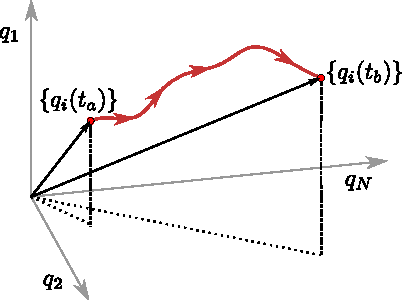
\includegraphics[width=0.5\textwidth]{images/fig_hamilton.pdf}	 
	\end{center}
	\caption{Trayectoria de un sistema mecánico $\{ q_i \}$ entre dos puntos del espacio $N$-dimensional de
	coordenadas generalizadas.}
	\label{principio_hamilton}
\end{figure}

En principio cualquier trayecto entre dos puntos es posible porque eso depende de la física a la cual está sometido
el sistema, no obstante existe un principio que permite saber cuál es la trayectoria que seguirá.

Considerando el lagrangiano $ \Lag = T - V $ y la siguiente integral (la acción $S$) entre los puntos $ \{ q_i(t_a) \} $
y $ \{ q_i(t_b) \} $,
\[
	S = \int_{t_a}^{t_b} \Lag( q_1(t, q_2(t), ..., \dot{q}_1(t),\dot{q}_2(t), ...,t )) \: dt
\]
se tiene que la trayectoria real entre estos dos puntos es tal que la integral $S$ toma su valor mínimo.

Dicho de otra manera, esto significa que $ S $ como funcional dependiendo de $ \{ q_i \}, \{ \dot{q}_i \} $
deberá tener un valor mínimo (o ser estacionaria) al especializarse en la trayectoria real.
Esto es análogo a lo que sucede en cálculo; en el mínimo de una función (de una o varias variables) la derivada 
se anula. El concepto equivalente en funcionales como $ S $ es el de variación nula.

La idea es construir una {\it variación} arbitraria respecto de la trayectoria real $ \{ q_i \} $ y forzar a que esa 
variación se anule para obtener un condición sobre las $ \{ q_i \} $ (para funciones esa condición era que el gradiente
se anule).

Si me sitúo en la trayectoria verdadera, es decir el conjunto $ \{ q_i(t) \}$, una variación arbitraria de la misma
tendrá la forma
\be
	q_i(t) \rightarrow q_i(t) + \delta q_i(t) \qquad i=1,2, ...
	\label{variacion}
\ee
donde cada coordenada $ q $ variará de acuerdo con su correspondiente desplazamiento $\delta q $.
La variación se hace en un intervalo de tiempo arbitrario $ [t_a,t_b] $ y con extremos fijos, 
\be
	\delta q(t_a) = 0 \qquad \qquad \delta q(t_b) = 0,
	\label{extremos_fijos}
\ee
lo que significa que los puntos de partida y llegada en el espacio de fases son los mismos.
\notamargen{Habría que justificar cuál es el significado de esto y porqué es así.}

Asimismo se pedirá que todas las trayectorias empleen el mismo tiempo de manera que la variación se hará en algún
tiempo fijo intermedio $ t_a < t < t_b $. O sea que $\delta t = 0$.

\notamargen{Cuán sketchi es todo esto!! Mucho para aclarar. Tal vez se justifique un minicurso de variacional como 
apéndice.}

Una representación unidimensional (una única $q$) puede verse en la Figura \ref{principio_accion_minima}.
La trayectoria real sería la curva $ q(t) $ en color rojo, mientras que la curva verde sería una trayectoria variada
a través de $ \delta q $. Los extremos fijos \eqref{extremos_fijos} implican que la variación es nula allí, y entonces
las curvas comienzan y terminan en el mismo punto.

\begin{figure}
	\begin{center}
	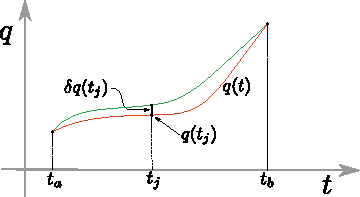
\includegraphics[width=0.7\textwidth]{images/fig_accion.pdf}	 
	\end{center}
	\caption{El principio de acción mínima}
	\label{principio_accion_minima}
\end{figure}

El hecho de considerar una variación a tiempo fijo $t_j$ implica que nos situaremos arbitrariamente en ese instante
y variaremos las trayectorias $ \{ q_i \} $ congeladas en ese instante arbitrario. Por supuesto, el resultado debería
valer para cualquier instante intermedio considerado.

La idea es determinar las condiciones que se necesitan para 
\[
	\frac{\delta S}{\delta q_i} = 0.
\]

Para ello comenzamos tomando una variación de $S$ que pasa dentro de la integral como 
\[
	\delta S = \int \left[ \Lag(q_i + \delta q_i, \dot{q}_i + \delta \dot{q}_i , t )
	- \Lag(q_i , \dot{q}_i , t ) \right] dt
\]
y donde vemos explícitamente que es a tiempo fijo.

La variación de la integral puede escribirse 
\[
	\delta S =  \int_{t_a}^{t_b} \sum_i^N \left( \dpar{\Lag}{\dot{q}_i} \delta \dot{q}_i +
	\dpar{\Lag}{q_i} \delta q_i  \right) dt,
\]
y como será útil tener todo en función de las variaciones $\delta q_i$, es conveniente expresar las variaciones $ 
\delta \dot{q}_i $ en términos de una derivada total a través de  
\[
	\frac{d}{dt}\left( \dpar{\Lag}{\dot{q}_i} \delta q_i \right) =
	\frac{d}{dt}\left( \dpar{\Lag}{\dot{q}_i} \right) \delta q_i + \dpar{\Lag}{\dot{q}_i}\delta \dot{q}_i,
\]
resultando en 
\[
	\delta S =  \int_{t_a}^{t_b} \sum_i^N \left[ \frac{d}{dt}\left( \dpar{\Lag}{\dot{q}_i} \delta q_i \right) -
	\frac{d}{dt}\left( \dpar{\Lag}{\dot{q}_i} \right) \delta q_i + \dpar{\Lag}{q_i} \delta q_i  \right] dt,
\]
que se puede separar en dos términos
\[
	\delta S =  \int_{t_a}^{t_b} \sum_i^N \left[ \frac{d}{dt}\left( \dpar{\Lag}{\dot{q}_i} \delta q_i \right) 
	\right] dt + \int_{t_a}^{t_b} \sum_i^N \left[ \dpar{\Lag}{q_i} - \frac{d}{dt}\left( \dpar{\Lag}{\dot{q}_i} 
	\right) \right]  \delta q_i \; dt,
\]

Pero el primer término es una derivada total y por el teorema fundamental del cálculo,
\be
	\int_{t_a}^{t_b} \sum_i^N \left[ \frac{d}{dt}\left( \dpar{\Lag}{\dot{q}_i} \delta q_i \right) \right] dt =
	\sum_i^N \left. \dpar{\Lag}{\dot{q}_i} \delta q_i \: \right|_{t_a}^{t_b}
\label{mc_borde_term}
\ee
y es nulo porque $\delta q_i=0$ en los extremos para toda coordenada $i$ (las variaciones son nulas en los extremos). 
Decimos que este es un término de superficie. Entonces la condición 
\[
	\delta S =  \sum_i^N  \int_{t_a}^{t_b}
	\left[ \dpar{\Lag}{q_i} - \frac{d}{dt}\left( \dpar{\Lag}{\dot{q}_i} \right)  \right]  \delta q_i  dt = 0
\]
se verificará por el cumplimiento de las ecuaciones de Euler-Lagrange\footnote{Como las variaciones $\delta q_i$ son 
arbitrarias e independientes la anulación de la ecuación $ \delta S $ requiere la anulación de cada uno de los 
$i=1,2,...N $ corchetes en los integrandos.}
\[
	\sum_i^N  \left[ \frac{d}{dt}\left( \dpar{\Lag}{\dot{q}_i} \right) - \dpar{\Lag}{q_i} \right] = 0.
\]

Se puede ver que 
\[
	\delta S = 0 \quad \iff \quad \sum_i^N  \left[ \frac{d}{dt}\left( \dpar{\Lag}{\dot{q}_i} \right) -
	\dpar{\Lag}{q_i} \right] = 0.
\]


Luego, si se hace $\Lag' = \Lag + df/dt$ (ambos lagrangianos difieren en una derivada total con 
respecto al tiempo) la trayectoria que minimiza $\Lag'$ es la que misma que minimiza
$\Lag$ por la condición dada por \eqref{mc_borde_term}. 

La moraleja es que si los lagrangianos difieren en una derivada total del tiempo obtenemos la misma
física.

% =================================================================================================
\section{Aplicaciones del principio de acción mínima}
% =================================================================================================

\[
	S = \int (T-V_0) dt
\]
donde el lagrangiano es con $V=V_0$ constante (un lagrangiano sujeto a potencial constante).
La integral de acción da una medida de la longitud de la órbita (el espacio recorrido).
Para una partícula sujeta a $V=0$
\[
	S = \frac{1}{2}\int m v_0^2 dt = \frac{1}{2}mv_0^2(t-t_0)
\]
de manera que $v_0(t-t_0)$ representa la distancia $d$ recorrida, y es 
\[
	S = \frac{1}{2}mv_0 d
\]

Comentario sobre el cálculo de las variaciones
\notamargen{Esta idea debe estar en el suplemento matemático que le dedicaremos a variacional}
\[
	I = \int f\left(x, \dtot{x}{t}, t\right) dt 
\]
entonces $I$ es extremo si
\[
	\frac{d}{dt} \left( \dpar{f}{[dx/dt]}\right) - \dpar{f}{x} = 0
\]
También podemos encontrar esta notación, dependiendo del tipo de problema,
\[
	I = \int f\left(y, \dtot{y}{x}, x\right) dx 
\]


% =================================================================================================
\section{Multiplicadores de Lagrange}
% =================================================================================================

Partimos de la acción
\[
	S = \int_{t_i}^{t_f} \Lag \left( q_i[t], \dot{q}_i[t], t \right) dt
\]
entonces 
\[
	\delta S = 0 \quad \Leftrightarrow \quad \int
	\sum_{j=1}^{N} \left[ \frac{d}{dt}\left( \dpar{\Lag}{\dot{q}_j} \right) -
	\dpar{\Lag}{q_j} \right]\delta q_j dt
\]
donde $\delta q_j$ son desplazamientos independientes. Si no se pued despejar alguna $\delta q_j$ (con 
vínculos no-holónomos, por ejemplo) entonces algún $\delta q_j$ es independiente de modo que para que 
valga $\delta S =0 $ necesitaré 
\[
	\sum_{\ell}^N a_\ell^k(q_i,t) \dot{q}_\ell + b^k(q_i,t) = 0
\]
que son los vínculos ($k=1,...,s$); son $s$ ecuaciones de vínculo.
Multiplicamos por $\delta t$ y vemos que no son independientes
\[
	\sum_{\ell}^N a_\ell^k(q_i,t) \delta {q}_\ell + b^k(q_i,t) \delta t= 0
\]

Sean $\delta q_\ell$ variación a $t$ fijo, entonces 
\[
	\sum_{\ell}^N a_\ell^k(q_i,t) \delta {q}_\ell
\]
\[
	\int_{t_i}^{t_f} \lambda^k \sum_{\ell}^N a_\ell^k(q_i,t) \delta {q}_\ell dt = 0
\]
recordando que $\ell$ suma en los grados de libertad. Podemos sacar la suma fuera,
\[
	\sum_{k}^s \int_{t_i}^{t_f} \lambda^k \sum_{\ell}^N a_\ell^k(q_i,t) \delta {q}_\ell dt = 0
\]
Absorbo la otra sumatoria en el segundo término y paso de $\ell \to j$.
\[
	\int  \sum_{j=1}^N \left\{ \frac{d}{dt}\left( \dpar{\Lag}{\dot{q}_j} \right) -\dpar{\Lag}{q_j}
	- \sum_{k}^s \lambda^k a_\ell^k(q_i,t) \right\} \delta {q}_\ell dt = 0
\]
entonces 
\[
	\sum_{j=1}^N \frac{d}{dt}\left( \dpar{\Lag}{\dot{q}_j} \right) -\dpar{\Lag}{q_j} =
	\sum_{j=1}^N \sum_{k}^s \lambda^k a_\ell^k(q_i,t) =  
	\sum_{j=1}^N \sum_{k}^s \lambda^k \nabla_j f^k \cdot \frac{\delta \vb{r}_j}{\delta q_j} 
\]
siendo $\nabla_j f^k $ el gradiente de la ecuación de víngulo respeco de $j$ y donde $\lambda^k$
es la fuerza de vínculo asociada al vínculo no despejado pues como la fuerza generalizada
(que no proviene de potencial)
\[
	Q_j = \sum_i^N \vb{F}_i^a \cdot \dpar{\vb{r}_i}{q_j}
\]
y comparando vemos que 
\[
	Q_j = \sum \lambda^k a^k_j(q_j,t) \quad \textrm{vínculos no holónomos}
\]
\[
	Q_j=  \sum \lambda^k \nabla_j f^k \cdot \delta \vb{r}_j  \quad \textrm{vínculos holónomos}
\]

En el caso de vínculos holónomos 
\[
	g(\vb{r}_1,...,\vb{r}_n,t) = 0 
\]
donde no quise despejar en función de $q_q,...,q_n$ resulta que 
\notamargen{El supraíndice con $\delta q_j$ va sobre el igual en realidad.}
\[
	Q_j^{\delta q_j} =  \sum_i^N \lambda (\nabla_i f^k\cdot\delta\vb{r}_i)
\]
donde $\delta\vb{r}_i$ es un desplazamiento virtual de la partícula.
Vamos a reescribir este término,
\[
	\sum_i^N \dpar{g^k}{\vb{r}_i} \delta \vb{r}_i = 0
\]
\[
	\nabla_i f^k\cdot\delta\vb{r}_i = \sum_i \dpar{g^k}{\vb{r}_i} \dpar{\vb{r}_i}{q_j} \delta q_j
\]
\[
	Q_j^{\delta q_j} =  \lambda \sum_k \dpar{g^k}{\vb{r}_i} \sum_j \dpar{\vb{r}_i}{q_j} \delta q_j
\]
luego como 
\[
	a^k_j \equiv \dpar{g^k}{\vb{r}_i}
\]
se sigue que los $\lambda^k$ son las fuerzas de vínculo.

En el caso de vínculos no holónomos $\lambda^k$ son las fuerzas de vínculo asociadas a los 
vínculos no retirados.

\[
	Q_j {\delta q_j} =  \sum \lambda^k (\nabla_i g^k\cdot\delta\vb{r}_i)
\]
\[
	Q_j =  \sum_k \lambda^k \dpar{g^k}{\vb{r}_i} \dpar{\vb{r}_i}{q_j}
\]
\[
	Q_j =  \sum_k \lambda^k \dpar{g^k}{q_j}
\]
entonces $\lambda^k=F^v$.

Como extra escribamos que para cada grado de libertad $j$ 
\[
	\dpar{\Lag}{q_j} - \frac{d}{dt}\left( \dpar{\Lag}{\dot{q}_j} \right) - \sum_k^s \lambda^k a_j^k \equiv 0
\]
donde $\delta q_j$ son ahora independientes.
\[
	Q_j = \sum_i^N F_i^a \dpar{\vb{r}_i}{q_j}. 
\]

\begin{ejemplo}{\bf Moneda rodando por un plano}
Consideramos una moneda que rueda libremente por un plano (no sujeta a potencial).
Situraemos un sistema de ejes sobre la moneda, que etiquetaremos 123 y otro fijo fuera
de la misma xyz.
\[
	\vb{V}_{cm} = -\vb{\Omega} \times \vb{r} =
	-(\dot{\phi}\hat{2} + \dot{\psi}\hat{3}) \times (-a\hat{2})
\]
\[
	\dot{x}\hat{x} + \dot{y}\hat{y} = -a \dot{\psi}\hat{1}
\]
siendo los vínculos
\[
	z_{cm} - a = 0 \qquad \theta=\pi/2 \qquad |\vb{V}_{cm}| = a\dot{\psi}
\]
de tal modo que son dos grados de libertad. El lagrangiano puede escribirse como 
\[
	\Lag = T = \frac{1}{2}m a^2 \dot{\psi}^2  + \frac{1}{2} I_2^2 \dot{\phi}^2 + \frac{1}{2} I_3^2\dot{\psi}^2.
\]
\notamargen{No entiendo/recuerdo lo que quise decir con la expresión {\it bajar los ejes}.
Calculo que se relaciona con la proyección de los ejes 123 en xyz. Confirmarlo.}

\begin{figure}
	\begin{center}
	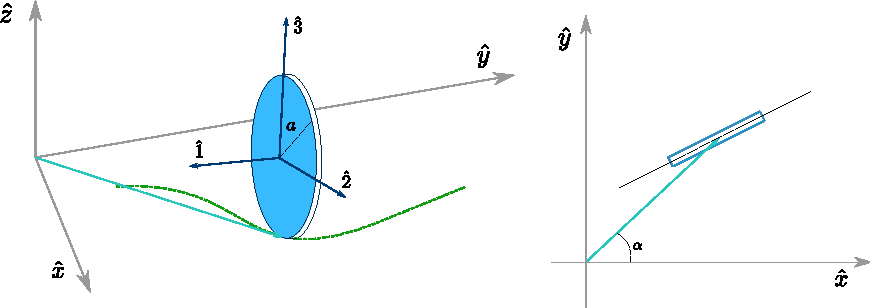
\includegraphics[width=0.4\textwidth]{images/fig_moneda.pdf}	 
	\end{center}
	\caption{Moneda que rueda libremente por un plano.}
\end{figure} 

Como los vínculos dependen de la velocidad, resulta 
\[
	\dot{y} = a\dot{\psi} \cos(\psi) \sin(\phi) = a \sin(\phi) \dot{\psi}
\]
\[
	\dot{x} = a\dot{\psi} \cos(\psi) \cos(\phi) = a \cos(\phi) \dot{\psi}
\]
de tal manera que 
\[
	\dot{y} - a \sin(\phi) \dot{\psi} = 0 \qquad \dot{x} - a \cos(\phi) \dot{\psi} = 0
\]
y luego esto equivale a 
\[
	\lambda_1(dy - a \sin(\phi) d\psi) = 0 \qquad \lambda_2(dx - a \cos(\phi) d\psi)= 0
\]
y finalmente 
\[
	\frac{d}{dt}\left(\dpar{\Lag}{\dot{q}_i}\right) - \dpar{\Lag}{q_i} =
	\lambda_i \nabla_i f \cdot \delta \vb{r}_i
\]
Podemos escribir
\[
	m \ddot{x} = \lambda_1 \qquad m \ddot{x} = m a \frac{d}{dt}( \cos(\phi)\dot{\psi} )
\]
\[
	m \ddot{x} = m a ( -\sin(\phi)\dot{\phi}\dot{\psi} + \cos(\phi)\ddot{\psi} )
\]
\[
	m \ddot{y} = \lambda_2
\]
\[
	I_2\ddot{\phi} = 0 \qquad I_3\ddot{\psi} = - \lambda_2 a \sin(\phi) -\lambda_1 a \cos(\phi)
\]
\[
	\hat{1} = \cos(\psi)[\sin(\phi)\hat{y} + \cos(\phi)\hat{x}]
\]

\label{moneda}
\end{ejemplo}

% =================================================================================================
\section{Potenciales dependientes de la velocidad}
% =================================================================================================

Hasta el momento se consideró que el potencial $V$ dependía únicamente de la posición y resultaba eso en
una fuerza generalizada [la llamé así?]
\[
	Q_j = -\dpar{V}{q_j}
\]
para la cual el $\Lag\equiv T-V$ cumplía las ecuaciones de Euler Lagrange
\be
	\dtot{}{t} \left( \dpar{\Lag}{\dot{q}_j} \right) - \dpar{\Lag}{q_j} = 0.
	\label{el-pot-x}
\ee

Si en cambio se tiene un potencial dependiente, además, de la velocidad,
\[
	U = U(q_1, ..., q_2,\dot{q}_1,...,\dot{q}_n,t ) 
\]
y se requiere que sigan valiendo las ecuaciones \eqref{el-pot-x} para $\Lag \equiv T-U$, necesitaremos evidentemente
\[
	Q_j = \dtot{}{t} \left( \dpar{U}{\dot{q}_j} \right)  -\dpar{U}{q_j},
\]
una fuerza generalizada que depende de posiciones y velocidades.

El ejemplo canónico de una tal fuerza es la fuerza de Lorentz, que es la que sufre una partícula de carga $q$ en
presencia de un campo electromagnético dado por campos $\vb{E}, \vb{B}$ y cuya forma es
\be
	\vb{F} = q \vb{E} + \frac{q}{c} ( \vb{v} \times \vb{B} )
	\label{f_lorentz}
\ee

Esta fuerza \eqref{f_lorentz} puede expresarse en términos de dos potenciales. Para ello es necesario recurrir a
las relaciones que verifican los campos $\vb{E}, \vb{B}$ y que están dadas por las ecuaciones de Maxwell, cuyo esquema 
se presenta en la siguiente tabla.
\begin{center}
\begin{tabular}{|c|c|}
\hline
& \\
$ \nabla\cdot\vb{E} = 4 \pi \rho $ & $ \nabla \cdot \vb{B} = 0 $ \\
& \\
$ \displaystyle \rotorm{E} = -\frac{1}{c} \dpar{\vb{B}}{t} $ &  
$ \displaystyle \rotorm{B} = \frac{4\pi}{c}\vb{J} + \frac{1}{c} \dpar{\vb{E}}{t} $ \\
 & \\
\hline
\end{tabular}
\end{center}

Dado que la divergencia de \vb{B} es nula, entonces existe un potencial vector \vb{A} tal que 
\[
	\rotorm{A} = \vb{B}.
\]
Entonces, la ley de Faraday resulta 
\[
	\rotorm{E} = -\frac{1}{c} \dpar{}{t} \left(\rotorm{A} \right) 
\]
o bien 
\[
	\nabla\times\left( \vb{E} + \frac{1}{c}\dpar{\vb{A}}{t} \right) = 0
\]

La cantidad entre paréntesis es de rotor nulo y entonces se puede escribir
\[
	\vb{E} + \frac{1}{c}\dpar{\vb{A}}{t} = -\nabla \vp( \vb{x}, t )
\]
de manera que los campos \vb{B}, \vb{E} pueden expresarse en términos de una función escalar $\vp$ y un campo vectorial
\vb{A} como
\[
	\vb{B} = \rotorm{A} \qquad \qquad \vb{E} = - \nabla \vp - \frac{1}{c} \dpar{ \vb{A} }{t} .
\]

Entonces, en términos de estos potenciales \eqref{f_lorentz} resulta 
\[
	\vb{F} = -q\nabla \vp - \frac{q}{c} \dpar{ \vb{A} }{t} + \frac{q}{c} \vb{v} \times \rotorm{A}.
\]

Supongamos, para simplificar el razonamiento, que es $ \vb{F} = F_x \hat{x} $ y veamos que 
\[
	F_x = -q \dpar{ \vp }{ x } - \frac{q}{c} \dpar{ A_x }{t} + \frac{q}{c} \left( v_y [\rotorm{A}]_z - v_z [\rotorm{A}]_y \right)
\]
se puede escribir
\[
	F_x = \dtot{}{t} \left( \dpar{U}{v_x} \right)  -\dpar{U}{x}.
\]

Desarrollando explícitamente el rotor se tiene 
\[
	\left( v_y [\rotorm{A}]_z - v_z [\rotorm{A}]_y \right) = 
	v_y \dpar{A_y}{x} - v_y \dpar{A_x}{y} - v_z \dpar{A_x}{z} + v_z \dpar{A_z}{x} + v_x \dpar{A_x}{x} - v_x \dpar{A_x}{x}
\]
donde se ha sumado y restado la conveniente combinación $ v_x \partial_x A_x $. Dado que las velocidades y las posiciones son variables
independientes (se verifica $ \partial_a v_b = 0 $ para cualquier combinación $ a,b=x,y,z $) se puede {\it filtrar} la velocidad dentro
de las derivadas para reescribir 
\[
	v_x \dpar{A_x}{x} + v_y \dpar{A_y}{x} + v_z \dpar{A_z}{x} = \dpar{}{x}( v_xA_x + v_yA_y + v_zA_z ) = \dpar{}{x}( \pe{v}{A} )
\]
% \[
% 	\left( v_y [\rotorm{A}]_z - v_z [\rotorm{A}]_y \right) = 
% 	\dpar{}{x}( v_xA_x + v_yA_y + v_zA_z ) - v_x\dpar{ A_x}{x} - v_y\dpar{A_x}{y} - v_z\dpar{A_x}{z}.
% \]
Los tres términos restantes en derivadas respecto de $A_x$ no son otra cosa que una derivada total,
\[
	- \frac{q}{c} \left(  \dpar{ A_x }{t}- v_x\dpar{ A_x}{x} - v_y\dpar{A_x}{y} - v_z\dpar{A_x}{z} \right) =
	- \frac{q}{c} \left( \dpar{ A_x }{t} - \vb{v}\cdot\nabla( A_x ) \right) = - \frac{q}{c} \dtot{A_x}{t}
\]

Luego, se fuerza la aparición de una derivada con respecto a la velocidad (para obtener una expresión en consonancia con la buscada)
del siguiente modo
\[
	A_x = \dpar{}{v_x}(v_xA_x + v_yA_y + v_zA_z) = \dpar{}{v_x}(\pe{v}{A}),
\]
y juntando todo resulta
% \[
% 	F_x = -q \dpar{ \vp }{ x } - \frac{q}{c} \dpar{ A_x }{t} + \frac{q}{c} \left( \dpar{}{x}( \pe{v}{A} )
% 	- v_i \partial_i\left( \dpar{}{v_x}(\pe{v}{A}) \right) \right)
% % 	- v_x \dpar{}{x}( \dpar{}{v_x}(\pe{v}{A}) ) - v_y \dpar{}{y}( \dpar{}{v_x}(\pe{v}{A}) ) 
% % 	- v_z \dpar{}{z}( \dpar{}{v_x}(\pe{v}{A}) ) \right).
% % 	
% \]
% donde el último término en el RHS representa la suma de tres. Reordenando esta expresión
\[
	F_x = -\dpar{ }{ x }\left( q\vp - \frac{q}{c} \pe{v}{A} \right) 
	+ \dtot{ }{t} \left( \dpar{}{v_x}\left( -\frac{q}{c}\pe{v}{A} \right) \right) .
\]

Como $\vp=\vp(\vb{x},t)$, se la puede incluir dentro de la derivada con respecto a la velocidad obteniendo finalmente el 
resultado buscado
\[
	F_x = -\dpar{ U }{ x } + \dtot{ }{t}\left( \dpar{U}{v_x} \right),
\]
donde 
\[
	U = q \vp - \frac{q}{c} \pe{v}{A}.
\]
 
\notamargen{Mucho para tener en cuenta: resumen previo de notación indicial, resumen de classical field theory. Aclarar
que posición y velocidad son independientes.}

Se puede demostrar directamente la fórmula anterior desde la expresión vectorial de \vb{F} utilizando su equivalente 
indicial, es decir a partir de
\[
	F_i = -q \partial_i \vp - \frac{q}{c} \:\partial_t A_i + \frac{q}{c} \: \epsilon_{ilm} v_l \epsilon_{mjk} 
	\partial_j A_k
\]
que es la coordenada $i$-ésima de la fuerza \vb{F}. Utilizando las propiedades del símbolo de Levi-Civita se tiene 
\[
	F_i = -q \partial_i \vp + \frac{q}{c} \left[  -\partial_t A_i  + (\delta_{ij}\delta_{lk} - \delta_{ik}\delta_{lj}) v_l \partial_j A_k \right]
\]
y, tras colapsar las deltas, y reordenar términos
\[
	F_i = -q \partial_i \vp + \frac{q}{c} \left[  -\partial_t A_i - v_j \partial_j A_i +  v_k \partial_i A_k  \right].
\]

Como el campo de velocidad \vb{v} no depende explícitamente de \vb{x} se puede introducir $v_k$ a través de la derivada $\partial_i$. Además los
dos primeros términos del corchete representan la derivada total de $A_i$ de manera que tenemos
\[
	F_i = -q \partial_i \vp + \frac{q}{c} \left[  - \dtot{}{t} \left(A_i\right)  + \partial_i (v_k A_k)  \right],
\]
o bien 
\[
	F_i = - \partial_i \left[ q\vp - \frac{q}{c}  (v_k A_k) \right] -  \dtot{}{t} \left( \frac{q}{c} A_i \right).
\]

Se puede hacer aparecer explícitamente lo faltante dentro de la derivada total notando que se puede escribir de manera absolutamente general
\[
	\frac{q}{c} A_i =  \dpar{}{v_i} ( - q\vp + \frac{q}{c} v_k A_k )
\]
dado que $\vp$ y $\vb{A}$ son funciones de la posición y el tiempo solamente. Luego,
\[
	F_i = - \partial_i \left[ q\vp - \frac{q}{c}  (v_k A_k) \right] + \dtot{}{t} \left[ \dpar{}{v_i} ( q\vp - \frac{q}{c} v_k A_k ) \right]
\]
y esto significa que el potencial completo es
\[
	U(\vb{x},\vb{v},t) = q \: \vp(\vb{x},t) - \frac{q}{c} \: \pe{v}{A}(\vb{x},t).
\]

En el ejemplo de la fuerza de Lorentz se desprecia el campo generado por la misma partícula que se mueve. Es decir, 
que el campo externo no es afectado por el movimiento de la partícula.
Una formulación lagrangiana que lo tuviera en cuenta debería considerar un $\Lag_p$ para la partícula.

% =================================================================================================
\section{Cambio de {\it gauge} en potenciales}
% =================================================================================================

Según se vio en la sección anterior, en el caso del electromagnetismo tenemos un potencial $ U $ que depende de la posición y la velocidad
de una manera muy especial. Además el potencial escalar $ \vp $ usual en la electrostática fue necesario definir un potencial vector \vb{A}
que estaba vinculado con el campo magnético \vb{B} a través de : $\rotorm{A}=\vb{B}$.

Solamente se le pide al campo \vb{A} que su rotor sea \vb{B} y esto no lo determina por completo. En particular si se define 
\[
	\vb{A}' = \vb{A} + \nabla f,
\]
un nuevo potencial $\vb{A}'$ que difiere del original por el añadido del gradiente de una función escalar, las ecuaciones de movimiento
no se ven alteradas. En efecto, la divergencia del campo magnético \vb{B} es
\[
	\divem{B} = \nabla \symbf{\cdot} (\rotorm{A}') = 
	\nabla \symbf{\cdot} (\rotorm{A}) + \nabla \symbf{\cdot} (\nabla \times {\nabla f}) = 0
\]
donde el cero se logra porque cada uno de los dos miembros es cero por separado.
Asimismo, como el rotor de un gradiente es nulo, el rotor de \vb{B} no se ve alterado;
\[
	\rotorm{B} = \nabla \times( \rotorm{A}' ) =
	\nabla \times( \rotorm{A} ) + \nabla \times ( \nabla \times \nabla f ) =
	\nabla \times( \rotorm{A} ).
\]

Luego, hay un grado de libertad extra en la determinación del \vb{A} que es esta función escalar $f$, y que se suele expresar
dando la divergencia de \vb{A}. En efecto, 
\[
	\divem{A}' = \divem{A} + \nabla^2 f.
\]

La divergencia de \vb{A} se puede elegir entonces arbitrariamente y esto es lo que se conoce como la {\it libertad de gauge}[?]
o el cambio de {\it gauge} del potencial. Descansa en el hecho de que las ecuaciones de movimiento son, por supuesto, independientes
del gauge elegido.
\notamargen{Chequear esta mini subsección.}


% Como ejemplo citamos \cite{einstein}.
% O bien \cite{example}.
% Tal vez \citep{Aspnes:1973}

% ============================================================================

% \bibliographystyle{CBFT-apa-good} % (uses file "apa-good.bst")
% \bibliography{CBFT.Referencias} % La base de datos bibliográfica


\end{document}
